
%% Is the line still missing in NM diagram when printed out?
%% Mention spatial stability? alpha,beta,gamma?
%% Discuss neutrality!
%% Adress network sampling more explcitly..(or next chapter? need to state how many iterations used..)

\section{Introduction}
\label{sec:methods_intro}
%% Check these references! (other chaptrs)
The research presented in this thesis represents an \emph{in silico} investigation of ecological community dynamics; how they respond to habitat loss and the role of species interactions. All of the experimental results, except for those at the beginning of chapter \ref{chap:interactions}, are generated using the same modelling framework. This modelling framework was previously developed by Lurgi, Montoya and Montoya \cite{lurgi2015effects}. In this chapter we provide the details of that framework; including how the model was previously used (section \ref{sec:lurgi_prev}); the procedure for generation of interaction network topologies (section \ref{sec:interaction_network}); the specification of the individual-based model (IBM) used for simulations (section \ref{sec:the_model}); and the two algorithms used to model habitat loss (section \ref{sec:model_HL}). We also outline the implementation of this framework in code (section \ref{sec:implementation}) and give examples of the dynamics generated by the IBM model (section \ref{sec:dynamics_results}). At the end of the chapter (section \ref{sec:metrics_explained}) we define the suite of ecological metrics and analysis methods that are used to characterise simulated communities throughout the thesis. This suite is not exhaustive. In particular additional analytic techniques are introduced in chapters \ref{chap:stress_testing} and \ref{chap:interactions}. However the methods defined in this chapter have all been used previously in empirical or theoretical ecology studies - together they represent a \emph{community ecology} toolbox. 

\section{Previous use of the model}
\label{sec:lurgi_prev}

The modelling framework outlined in this chapter is largely the same as that presented in \cite{lurgi2015effects}. The model specification provided here is more detailed than in that paper, and is mostly in original wording. Where material is reproduced from \cite{lurgi2015effects}, it is cited explicitly. The fundamentals of the model remain unchanged, and the implemented code is largely reused with minor amendments (see section \ref{sec:implementation}). The novel elements of the modelling presented in this thesis are: 1) the implementation of habitat loss algorithms (section \ref{sec:model_HL}); and 2) the exploration of new model parameter values.

In \cite{lurgi2015effects} the authors use the model to study the effects of increasing levels of mutualism on the stability of simulated communities. The communities are multi-trophic food webs, in which some fraction of the atagonistic links between the bottom two trophic levels are replaced by mutualistic links (section \ref{sec:link_replacement}). This link replacement alters the behaviour of the corresponding species by making them mutualistic (either plant or animal mutualists). The authors consider multiple aspects of community stability. Namely, temporal variability, spatial variability, spatial aggregation and interaction strengths (section \ref{sec:def_stability_metrics}). The study found that increasing levels of mutualism increased stability in some respects, but had no significant effect in other respects. Specifically, higher mutualism was associated with greater spatial aggregation and weaker interactions, but did not change either temporal or spatial variability. Furthermore, mutualism was seen to increase the total number of individuals in a community, while reducing diversity and producing few changes in structural network properties. The reduction in diversity was attributed to the dominance of mutualistic species, which accounted for the increased overall abundance. The only network properties that significantly changed were \emph{generality} and \emph{specialisation} (section \ref{sec:define_network_metrics}), which both decreased. In the case of generality this was attributed to changes in the relative abundances of prey, while the change in specialisation was argued to result from the overall reduction in interaction strengths. We do no provide a detailed discussion of these results here, since it can be found in \cite{lurgi2015effects}. However these previous findings provide some context for the current investigation.  

%Higher mutualism was . The authors argued that high spatial aggregation results in reproductive stability because it makes it easier for individuals to find a mate (although this link is not explicitly tested).  
% In general it was seen that increasing the level of mutualism in simulated communities increased their stability. 

%We discuss standard interpretations and draw comparisons with other studies where relevant\footnote{Here, or in analysis?}. 

%\section{Agent based simulation}
%\label{sec:method}
%To simulate habitat loss, a fraction of the grid cells are made inhospitable to all species. We compare two algorithms for choosing which cells to destroy: 1) random destruction and 2) contiguous destruction. For random destruction grid cells are destroyed uniformly at random, up to the desired fraction of the total landscape. For contiguous destruction a seed cell is chosen uniformly at random, then destruction spreads radially in all directions from this point.  
%We simulated communities with MAI values of $0, 0.1, 0.2,..., 1.0$, with habitat loss (HL) percentages of $0, 10, 20, ...,90$. For each combination of MAI and HL values, 25 replicates were simulated with different interaction networks (same species richness, same connectance).


\section{The interaction network}
\label{sec:interaction_network}

Before we can simulate community dynamics we need to define the network of interactions between the species. We refer to this as the \emph{underlying interaction network} because it defines the potential for interactions in the IBM. If two individuals meet, and they belong to species that share a link in the underlying network, they may interact. This is in contrast to the \emph{realised interaction network}, which is simply the network of all interactions that actually occur between members of species during a given period of time. As motivated in section \ref{sec:intro_interactions}, the inclusion of multiple interaction types in the model is a key feature of this research. Therefore we require underlying interaction networks that contain both \emph{antagonistic} (predator-prey) and \emph{mutualistic} (plant-pollinator) links. This allows individuals to interact either via predation or mutualism depending on the type of link that they share. Additionally the networks must be multi-trophic since we wish to study whole community patterns and responses. It would be possible to use empirically derived topologies for the underlying network. Indeed there is some precedent for this in simulation studies \cite{fortuna2013habitat}. However we use a method, pioneered by Lurgi et al. \cite{lurgi2015effects}, to generate artificial network topologies with desired properties. The method first creates an artificial food web (section \ref{sec:niche_model}), and then replaces some of the links to introduce mutualism between some species in the first two trophic levels (section \ref{sec:link_replacement}). The strength of this approach is that it allows us to specify the ratio of mutualistic to antagonistic interactions between species in the first two trophic levels, whilst controlling the total number of species (S) and the connectance (C) of the network. Therefore we are able to vary the level of mutualism and determine the effect that this has on community responses to habitat loss. 

%Unlike most previous \emph{in silico} studies, the model includes both trophic and mutualistic interactions. Species belong to four trophic levels. The niche model generates a trophic interaction network. Then a fraction of the links between species in the first two trophic levels are changed to define mutualisms ($-+ \rightarrow ++$). The fraction of links switched is called the mutualistic vs. antagonistic interaction (MAI) ratio.  
%An underlying interaction network defines which direct interactions between species are allowed. This network contains two types of link: . To construct this network a food web, containg only antagonisitc links, is generated using the niche model (section \ref{sec:niche_model}). This network cosists of 60 species belonging to 4 trophic levels, with links that define the feeding relationships between them. Species in the basal trophic level represent plants and those in the trophic level above represent herbivores. To introduce mutualism a fraction of the herbivorous links are replaced by mutualistic links (section \ref{sec:link_replacement}). 


\subsection{The niche model}
\label{sec:niche_model}

% More references for niche mdoel shown to prduce realistic webs....

The niche model (NM) of Williams \& Martinez \cite{williams2000simple} is used in the first stage of network generation to create artificial food webs. The model was first published in 2000 and it was shown to produce networks with statistical properties similar to empirical food webs. Since that date numerous competing models have been proposed \cite{stouffer2005quantitative} to explain to structure of complex food webs. However the NM has been shown to outperform the other methods in the generation of \emph{realistic} food web topologies \cite{williams2008success}, and has proven a useful tool for the creation of artificial networks in theoretical studies such as our own \cite{c2008food,dunne2002food,staniczenko2010structural,lurgi2015effects}. Part of the attraction of the model is its simplicity - species are randomly distributed along a one-dimensional trophic niche, and are then assigned to consume all other species that fall within a certain region of the niche space. The details of the procedure are as follows. 

The model has two parameters: the number of species S, and the desired connectance C. The model output is a binary adjacency matrix $\mathbf{a}$ that the defines the presence/absence of links between species. The element $a_{ij} = 1$ implies that species $i$ consumes species $j$, and $a_{ij} = 0$ implies the absence of an interaction. Connectance is defined as the proportion of the maximum possible number of links that are realised i.e. $C = L/S^2$, where $L$ is the number of links in the network.

\begin{figure}
	\centering
	\includegraphics[width=\textwidth]{"diagrams/niche_space"}
	\caption[Niche space.]{A representation of 1-dimensional \emph{niche space} as visualised in the original publication \cite{williams2000simple}, for number of species $S=6$. The blue triangles represent the placement of species in niche space. The \emph{niche value} of species $i$ is given by $n_i$. The width and centre of the \emph{feeding range} for species $i$ are denoted by $r_i$ and $c_i$ respectively. Species $i$ consumes all species whose niche values fall within its feeding range, here $j$ and $k$.}
	\label{fig:niche_model}
\end{figure}


Figure \ref{fig:niche_model} illustrates the concept of niche space, and shows the niche value $n_i$ and feeding range $r_i$ for a particular species $i$. Niche space is the 1-dimensional range of real numbers $[0,1]$. Each of the $S$ species is assigned a niche value $n_i$, drawn uniformly at random from the niche space. The species is then assigned a feeding range with a central value $c_i$ and a width $r_i$. Species $i$ consumes all species, including itself, whose niche values fall within its feeding range. To determine the width of the feeding range, a beta function with expectation $2C$ is used to draw a number $x_i$ from the range $[0,1]$. This number is then multiplied by the species niche value $n_i$ to give the feeding range width: $r_i = x_i \times n_i$.  Since $n_i \sim U(0,1)$, we know that the expectation value $E(n_i) = 0.5$, and so $E(r_i) = C$. Therefore on average each species consumes a fraction $C$ of the total number of species, resulting in a network with close to the desired connectance (an approximation that improves for larger number of species). The only departure form the above is for the species with the smallest niche value $n_i$, which is assigned a zero-width feeding range $r_i = 0$. Therefore this species consumes no others, and there is guaranteed to be at least one basal species in the web.

A beta function has two parameters: $\alpha, \beta \in \mathbb{R^+}$. The choice of $\alpha = 1$ simplifies the probability density function to:

\begin{equation*}
f (x; 1,\beta) = \begin{cases}
\beta (1-x)^{\beta - 1} &\mbox{ if } 0 < x < 1,  \\
0	                    &\mbox{ otherwise. }
\end{cases}
\label{eq:beta_pdf}
\end{equation*}
%
The cumulative distribution function is derived by:
\begin{eqnarray*}
P(x) &=& \int_{0}^{x} \beta (1-x')^{\beta - 1} dx' \\
     &=& 1 - (1-x)^\beta . 
\label{eq:beta_cdf}                         
\end{eqnarray*}
%
Therefore, by choosing a probability value $y$ uniformly at random from the interval $[0,1]$, we can draw an $x$ value form our beta distribution:
 
\begin{eqnarray*}
y &=&  1 - (1-x)^\beta, \qquad \text{such that} \\[5pt]
x &=&  1 - (1- y)^{1/\beta}.                          
\label{eq:beta_sampling}
\end{eqnarray*}
%
The expectation value of this beta distribution is given by $E (x) = \frac{1}{1 + \beta}$, therefore we choose

\begin{equation*}
\beta = \frac{1}{2C} - 1
\label{eq:beta_value}
\end{equation*}
%
to give the desired expectation of $E(x) = 2C$.

Once the width $r_i$ has been chosen, the feeding range is placed in niche space by drawing the range centre $c_i$ uniformly at random from the interval $[r_i/2, n_i]$. Therefore cannibalism and looping are possible because up to half of the feeding range may contain niche values $\geq n_i$. In some cases the generated network may not be connected (i.e. contains one or more disconnected components), or two species may be trophically identical (i.e. have the exact same links as another species). In these cases the guilty species are deleted and reassigned new niche values ($n_i ,r_i,c_i$) until the resulting network is connected and without identical species. 

\begin{figure}
	\centering
	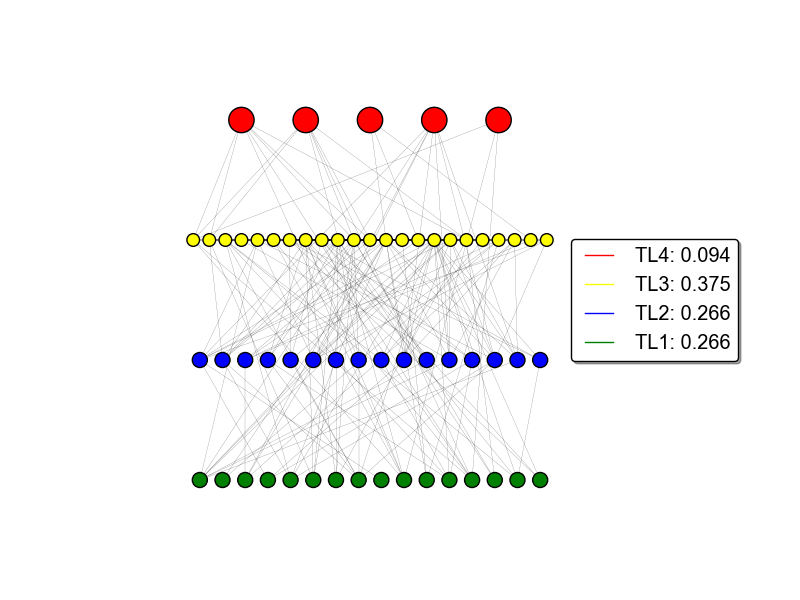
\includegraphics[width=\textwidth]{{{random_plots/example_food_web}}}
	\caption[A sixty species food web.]{An example food web of 60 species, generated using the niche model with trophic constraints (described in the text). Numbers given in the legend are the fraction of species belonging to each trophic level.}
	\label{fig:example_food_web}
\end{figure}


\subsection{Trophic constraints}
\label{sec:trophic_constraints}

As alluded to previously the niche model produces multi-trophic food webs. Specifically the resulting networks have four trophic levels (see figures \ref{fig:example_food_web},\ref{fig:trophic_cartoon}). The first trophic level consists of basal species, which have no prey and therefore represent plants. The second trophic level comprises species which feed only on plants. Therefore these species represent animals which are either strictly herbivorous, or may in fact be mutualists (see section \ref{sec:link_replacement}). The third trophic level contains species which feed on other animal species, but which are also predated upon by other animals. These species may also feed on basal species, in which case they represent omnivores. The fourth trophic level contains species which feed on animal species, but which have no predators of their own. Therefore these species represent top-predators. It is worth noting here that the niche model does not require top-predators to be strictly carnivorous. Therefore top-predators may happen to be omnivorous, feeding both on basal and non-basal species. We address this artefact of the niche model later in chapter \ref{chap:stress_testing}.

The niche model gives us control over the number of species and the connectance. However the proportion of species belonging to each trophic level cannot be specified. Williams and Martinez \cite{williams2000simple} showed that on average the of proportion of species belonging to basal, intermediate (levels two and three) and top trophic levels closely match those proportions found in empirical webs. However this is an ensemble statistic and so does not guarantee proportions for an individual web. Furthermore it is known that the niche model, and other food web assembly models, significantly underestimate the number of herbivore species\cite{williams2008success}. That is, although the number of intermediate species may be `correct', there are often too many species in the third trophic level and not enough in the second. To ensure that all the networks we generate contain a reasonable distribution of species across trophic levels we impose \emph{trophic constraints}. We stipulate that at least $25\%$, $25\%$ and $5\%$ of species must belong to the first, second and fourth trophic levels respectively. If the niche model output does not meet these constraints the network is rejected and we generate another. The percentages used were determined heuristically in the development of the model by Lurgi et al. \cite{lurgi2015effects}. They ensure that there is always sufficient species richness at each level, especially at the base of the web, and that the community is not dominated by the third trophic level. An example of a niche model network which meets the trophic constraints is shown in figure \ref{fig:example_food_web}.

\subsection{Link replacement}
\label{sec:link_replacement}

The second stage in network creation, having obtained a food web from the niche model, is to introduce mutualistic interactions. This is done by replacing some of the links between species in the first two trophic levels i.e. between plants and herbivores. This changes the way that some species interact from antagonism to mutualism (see section \ref{sec:CA_rules}). The fraction of these links switched is defined as the \emph{mutualistic vs. antagonistic interaction ratio} (hereafter MAI ratio). Figure \ref{fig:trophic_cartoon} is a schematic of a possible interaction network generated by this procedure, for a nineteen species community. In this case there are twelve links between the first two trophic levels, and six of these have been replaced by mutualistic links. The other six links remain antagonistic. Since half of the basal links have been replaced, the MAI ratio for this community is $0.5$.

%The mutualistic interactions are trophic, as with antagonisms, since there is an energy flow from resource to consumer. For example pollinators receive nectar from flowering plants. However in a mutualistic interaction there is a benefit for both parties. In this example flowering plants are pollinated and can reproduce. In the simulation model the plants recieve better dispersion abilities as a result of mutualisms 
%We impose the constraint that mutualisms can only exist between species of the first two trophic levels: plants and herbivores. Some of the antagonistic links between the first two trophic levels are replaced by mutualistic links. This changes the rules of interaction between individuals of these species in the cellular automata model (section \ref{sec:CA_rules}).


\begin{figure}
	\centering
	\includegraphics[width=0.6\textwidth]{"diagrams/trophic_cartoon"}
	\caption[Schematic of interaction network, with mutualism.]{Schematic of an underlying interaction network (reproduced from \cite{lurgi2015effects}). Nodes correspond to species, and arrows to trophic links (antagonistic or mutualistic) from resource to consumer. The six \emph{functional groups} of species are colour coded, and named in the legend. In this case there are twelve links between the first two trophic levels, six of these have been replaced by mutualistic links giving a MAI ratio of $0.5$. Mutualistic plants and animal mutualists are defined by any species that has \emph{at least} one mutualistic link. However species in both these groups may also have antagonistic links.}
	\label{fig:trophic_cartoon}
\end{figure}

The result of link replacement is a hybrid network that defines two types of interaction between species (although only one between any given pair). We can identify two functional groups in each of the first two trophic levels, based on the way species interact. In the first trophic level \emph{non-mutualistic plants} are basal species which do not have any mutualistic links. This group represents wind-dispersed plants which only have antagonistic interactions with the trophic level above. \emph{Mutualistic plants} are any basal species with at least one mutualistic link. This group are dispersed by species from the second trophic level via their mutualistic interactions and can no longer be wind dispersed. They may also be predated upon by herbivores, if they have such links. Similarly \emph{herbivores} are members of the second trophic level which only predate on basal species, whereas \emph{animal mutualists} are any species in the second trophic level with at least one mutualistic link. The top two trophic levels represent distinct functional groups, which we refer to as \emph{primary predators} and \emph{top predators}. See figure \ref{fig:trophic_cartoon} for a visualisation of these functional groups. 

For most of the results presented networks were generated with eleven different MAI ratios in the range: $[0,0.1,0.2,...,1.0]$. Communities with MAI$=0.0$ contain no mutualism, whereas those with MAI$=1.0$ contain only mutualistic interactions between the first two trophic levels. This is in accordance with the previous study \cite{lurgi2015effects}, and allows us to look at how communities with different MAI ratios respond to habitat loss. 


\section{Individual-based model}
\label{sec:the_model}


Community dynamics is simulated using a spatially explicit, individual-based model (IBM) that was developed by Lurgi et al. \cite{lurgi2015effects}. The landscape consists of a homogeneous two-dimensional lattice ($200 \times 200$ cells) on which individuals move around and interact subject to bio-energetic constraints. The lattice has periodic boundary conditions such that the topology of the landscape is toroidal. Each lattice cell has a space for an \emph{inhabitant} and a \emph{visitor}, such that a cell may contain at most two species. Basal species may only occupy the inhabitant space, whilst all other species may occupy either or both spaces. Distance on the lattice is defined as follows. The immediate neighbours of any given cell are the eight adjacent cells, including diagonals (i.e. a Moore neighbourhood). These eight neighbours are distance-1 from the central cell, whilst the sixteen cells surrounding them are distance-2, and so on (see figure \ref{fig:IBM_motion}). This distance metric is used in the rules for movement and reproduction (section \ref{sec:CA_rules}), the habitat loss algorithms (section \ref{sec:model_HL}), and also in the calculation of the spatial metrics (section \ref{sec:def_spatial_metrics}).

%% Notes (TODO):
% Ensure figures are referenced, and state this the follwoing is partly taken from the publication.
%% questions to confirm with Miguel
% Where does this model for mutualism come from?
% What energy are new plants created with in both types of asexual reproduction? Do the parents lose energy?

%TALK ABOUT HOW THIS MODEL DIFFERS FROM PREVIOUS MODELS? (MAYBE INTRO.)


The model has a large parameter space - there are seventeen free parameters, which are defined in table \ref{tab:IBM_parameters}. A discussion of the values chosen for these parameters can be found in section \ref{sec:parameters}. Initial conditions are defined randomly by the following procedure. For each cell in the landscape an individual belonging to a randomly selected basal species is placed in the inhabitant space, so that all cells contain a plant individual. Then individuals from randomly selected non-basal species are placed in the visitor space of randomly selected cells, until the desired fraction of the landscape (given by parameter \emph{OCCUPIED\_CELLS}) is filled with animal individuals. The simulation is then run for a given number of time steps following the local rules described in section \ref{sec:CA_rules} below.

%Table  shows all the model parameters, their values and definitions. Where possible the parameters values are chosen to be biologically realistic. 


\begin{figure}
	\centering
	\includegraphics[width=0.3\textwidth]{"diagrams/IBM_movement"}
	\caption[Motion of individuals.]{The trajectories of two individuals over 12 time steps are shown in \emph{black} and \emph{dark grey}. The distance-1 neighbourhoods of the two individuals on the first time step are shown in \emph{light grey}. Figure reproduced from \cite{lurgi2015effects}.}
	\label{fig:IBM_motion}
\end{figure}


\subsection{Local rules}
\label{sec:CA_rules}

The following local rules define the behaviour of individuals, which together generate the global dynamics of the IBM. In what follows capitalised-italicised words refer to model parameters, which are defined in table \ref{tab:IBM_parameters}. Each individual stores energy (or resource), which it expends to perform actions. Initially all individuals are given a random amount of energy between \emph{MIN\_RESOURCE} and \emph{MAX\_RESOURCE}. If the energy of an individual drops below \emph{MIN\_RESOURCE} it dies and is removed from the landscape. On each time step an initial cell is randomly selected and all cells are updated sequentially, starting at the initial cell. Cell update consists of the following ordered processes which occur first for the visitor individual and then for the inhabitant:

\begin{enumerate}
	\item Immigration
	\item Death
	\item Movement
	\item Reproduction
	\item Feeding
	\item Metabolic loss
\end{enumerate}

\subsubsection*{1) Immigration}
An immigrant individual is created with probability given by \emph{IMMIGRATION}. The species of the immigrant is selected uniformly at random from the original species pool. There must be space in the cell for the immigrant to be placed, or the immigrant must be able to feed upon the species present in the cell (in which case it does so and replaces it). Otherwise the immigrant is discarded. If placed, the immigrant is given a random starting energy.  
\subsubsection*{2) Death}
If the energy of an individual in the cell has fallen below \emph{MIN\_RESOURCE}, it is removed from the landscape.

\subsubsection*{3) Reproduction}
An individual may only reproduce if its stored energy is greater than \emph{MATING\_RESOURCE}. This is true for all species. Animals reproduce sexually, plants reproduce asexually.
\begin{itemize}
	\item \textbf{Sexual reproduction}: If an individual's energy exceeds \emph{MATING\_RESOURCE} it searches its distance-3 neighbourhood. If it finds an individual of the same species, with sufficient energy to mate, and it finds a destination cell with space for an animal (inhabitant or visitor space), then mating occurs. Both parents give a fraction of their stored energy (\emph{MATING\_ENERGY}) to the offspring, which is placed in the destination cell. If an individual has reproduced it carries out no further actions on that time step.
	\item \textbf{Asexual reproduction}: This occurs for plants via two possible mechanisms. 
	\begin{enumerate}
	\item If the individual is a non-mutualistic plant it reproduces with a probability equal to \emph{REPRODUCTION\_RATE}. If reproduction occurs the offspring is placed in a randomly selected available cell in the distance-3 neighbourhood. For plants, available means empty or only occupied by an animal individual. If no cells are available the plant cannot reproduce. Again a fraction of the parent plant's stored energy (\emph{MATING\_ENERGY}) is given to the offspring.
	\item Mutualistic dispersal occurs for mutualistic plants. This action is carried out by the animal partner, and is done in the `feeding' phase (see 5). The 'seed' of the parent plant is carried by the animal partner, so it may be placed beyond the distance-3 neighbourhood. 
    \end{enumerate}	 
\end{itemize}

\subsubsection*{4) Movement}
If the individual is a plant it does not move. Otherwise a neighbouring cell (distance-1) is selected uniformly at random. If the selected cell contains a prey species, feeding occurs (see 5). Otherwise, if there is an available space in the selected cell, the individual moves there. The motion is therefore a two-dimensional random walk, as represented in figure \ref{fig:IBM_motion}.
\subsubsection*{5) Feeding}
Having selected (in 4) to move into a cell containing prey, there are three possible trophic interactions:

\begin{enumerate}
	\item \textbf{Predation}: If neither individual belongs to a basal species a predation event occurs with probability \emph{CAPTURE\_PROB}. The prey species dies and a fraction of its energy \emph{EFFICIENCY\_TRANS} is given to the predator. The predator moves into the new cell.
	\item \textbf{Herbivory}: If one individual is a non-mutualistic animal, the other is a plant, and there is space to move into the selected cell, they interact. A fraction of the plant's energy \emph{HERB\_FRACTION} is lost, and a fraction (\emph{HERB\_EFFICIENCY}) of this energy is given to the herbivore. Both individuals continue living and the herbivore moves into the new cell. If the animal is an omnivore an additional trade-off (\emph{OMNI\_TRADEOFF}) is applied to its energy gained, since omnivores are less efficient at digesting plant matter than straight herbivores.   
	\item \textbf{Mutualism}: If the individuals share a mutualistic link, and there is space for the animal to move,they interact. A fraction of the plant's energy (\emph{MUT\_FRACTION}) is transferred to the animal. The animal also keeps track of which plant it interacted with. If it later reaches an available cell in the landscape it creates a new individual belonging to this plant species, with probability \emph{MUT\_EFFICIENCY}. On each time step that an offspring is not produced, the mutualistic efficiency is reduced by a fraction \emph{MUT\_COOLING}.  
\end{enumerate}  

\subsubsection*{6) Metabolic loss}
If the individual is an animal it reduces its stored energy by a fraction \emph{LIVING\_EXPEND}, to account for metabolic losses. If the individual is a plant it auto-trophically increases its energy by a fraction \emph{SYNTHESIS\_ABILITY}. This, along with the randomly generated immigrants, are the only energy input to the system.


\subsection{Model Parameters}
\label{sec:parameters}

A complex model such as this may display great variation in output depending on parameter values. During the model development by Lurgi et al. \cite{lurgi2015effects} a set of parameter values were selected that produced \emph{realistic community patterns} and stable dynamics (see section \ref{sec:dynamics_results}). In particular the rank-abundance (see section \ref{sec:define_rads}) and degree-distributions were shown to be well fitted by log-normal and exponential functions, which is a pattern that has been observed in natural communities \cite{montoya2006ecological}. Where possible these parameters are based on \emph{ecological realism}; the main example being trophic assimilation efficiency. It is well known that energy is lost when transferred between trophic levels, and that transfer rates are different depending on the type of resource consumed (plant vs. animal biomass) \cite{ings2009review}. As such the assimilation rate is higher for plant biomass than animal biomass (\emph{HERB\_EFFICIENCY} $>$ \emph{EFFICIENCY\_TRANS}). The extra reduction in transfer efficiency \emph{OMNI\_TRADEOFF} models the fact that omnivores are less well adapted to consume plant material because they also consume meat. Other than the omnivory trade-off all species within a functional group have identical parameters, and therefore differences between species are defined only by feeding relationships.

A key mechanism, and novel feature of the model, is mutualism. Mutualistic interactions are trophic, so energy is transferred from plant to consumer, but less than in a herbivorous interaction (\emph{MUT\_FRACTION} $<$ \emph{HERB\_FRACTION} $\times$ \emph{HERB\_EFFICIENCY}). Therefore a mutualistic animal benefits energetically from the interaction, but less so than if it were herbivorous. A mutualistic plant benefits significantly by having less of its resource consumed, and receiving improved dispersal ability. There is a potential disadvantage to the plant that it must wait for a partner to reproduce. However the combined effect is that mutualism shifts some of the benefit of interaction in favour of the plant, whereas herbivory only benefits the consumer and harms the plant.  

Lurgi et al. conducted a sensitivity analysis, which showed that their results were not significantly affected by a $\pm 10\%$ variation in the value of all parameters (see S.I. for \cite{lurgi2015effects}). Given the extensive effort that went into finding a stable and interesting region of parameter space, we choose to begin the investigation of habitat loss by using the same parameter values. These values, hereafter referred to as the \emph{default values}, are given in table \ref{tab:IBM_parameters}. In chapters \ref{chap:stress_testing} and \ref{chap:varying_immigration_rate} we explore the effect of varying certain parameters, with particular focus on the immigration rate.

%The model paramerts were chosen blalblabla... reference Ings et al. Which parameters are most interesting, why? Also discuss sensitivity analysis from previous publications, findings. We I conduct my own version? With regard to which parameters? (Maybe discuss this lat bit somehwere else).

\begin{table}[hp!]
\centering
%\begin{figure}	
\includegraphics[width=0.9\textwidth]{"tables/IBM_parameters"}
%\end{figure}
\caption[Default parameter values.]{Definitions of model parameters, and \emph{default values} used. Reproduced from \cite{lurgi2015effects}.}
\label{tab:IBM_parameters}
\end{table}

\section{Modelling habitat loss}
\label{sec:model_HL}

In order to study the effect of habitat loss (HL) on simulated communities we extend the IBM of Lurgi et al. \cite{lurgi2015effects} by implementing two habitat loss algorithms. Simulations are set up and run as detailed in the previous sections but on the 1000$^{th}$ time step, after the initial transience (see section \ref{sec:dynamics_results}), a given fraction of the lattice cells are destroyed. The individuals inhabiting the destroyed cells are removed. Subsequently an individual may select a destroyed cell to move into (see section \ref{sec:CA_rules}), in which case it is unable to move and remains in place. In the reproduction phase destroyed cells are counted as unavailable for the placement of offspring. Throughout the thesis results are presented for incrementally affected landscapes, representing a gradient of habitat loss. The levels of destruction are referred to by the percentage of destroyed cells: HL $=[0,10,20,..,90] \%$. The cells to destroy are chosen by two simple algorithms, giving two habitat loss scenarios: 1) Random and 2) Contiguous. These scenarios represent two extremes of the spatial pattern in which we may expect habitat to be destroyed in nature (see section \ref{sec:intro_habitat_loss}).

\paragraph*{1) Random habitat loss} proceeds by selecting lattice cells uniformly at random from the set of non-destroyed cells. This is repeated until the desired percentage HL is achieved. The result is a patchy and fragmented landscape.  

\paragraph*{2) Contiguous habitat loss} proceeds by selecting a `seed cell' uniformly at random from the pristine landscape. Destruction then spreads radially outwards form the seed cell, according to the distance metric defined in section \ref{sec:the_model} and the toroidal boundary conditions of the lattice. This results in contiguous regions destroyed and pristine habitat.
 

\section{Implementation}
\label{sec:implementation}

The code for the simulation model was originally written by Miguel Lurgi for research leading to the publication \cite{lurgi2015effects}. He and Daniel Montoya were responsible for the bulk of the model development, testing and parameter selection - a considerable task. My task was to take this `legacy code' and apply it to a study of habitat loss. The model is implemented in \emph{Python} \cite{python}, with several switches that ensure portability between different versions of the language. The programme makes extensive use of \emph{numpy} and \emph{networkx}, amongst other \emph{Python} libraries. A change in the return value of some methods in \emph{networkx} (specifically some methods from v1.9 return \emph{generator} objects, whereas in v1.7 they return \emph{lists}) forced me to make some amendments to the code. During this process I profiled the code using \emph{cProfile} and \emph{pstats}, because I noticed it was running very slowly. I determined that the cause was repeated calls to methods of the \emph{networkx} library, which were made every time an interaction needed to be checked in the network (for example to see if two individuals are able to interact). By storing two representations of the network - one as a \emph{networkx} object and one as a simple \emph{numpy} array - I was able to speed up the simulations by almost an order of magnitude. The \emph{networkx} methods need only be called when some network metric needs to be calculated. Having made the above changes I ran an ensemble of test simulations. Cross-checking the results with those in \cite{lurgi2015effects} confirmed that the simulations were behaving as expected.    

The original code was well written to be extendible, and there was a prototype algorithm for contiguous habitat loss. Therefore my job of implementing and testing the habitat loss algorithms (section \ref{sec:model_HL}) was made easy. I also added methods to save the spatial state of the system. This allows for \emph{post-hoc} spatial analysis, and also facilitated the creation of spatial animations of the evolution of the system (see animations at \cite{mcwilliams2015anim}, and figure \ref{fig:spatial_state_mai0.5}). All results presented in this thesis are from simulation ensembles run on \emph{Blue Crystal Phase 3} \cite{BC3}, the university's high performance computer cluster. Ensembles were run as parallel job arrays, and output saved in pre-constructed directory trees. I conducted post-simulation analyses in the statistical package \emph{R} \cite{Rlanguage} and in \emph{Python} making extensive use of the \emph{open source} libraries available.


\section{Dynamics of the model}
\label{sec:dynamics_results}

In the absence of habitat loss the dynamics of the model is characterised by an initial period of transient dynamics, with high amplitude oscillations, after which the populations settle into a \emph{relatively steady state}. A typical example of the population dynamics, aggregated by trophic level (TL), is shown in figure \ref{fig:example_model_dynamics}. The simulation that produced this figure used default parameters, and no habitat loss. In general we observe that the main transience, characterised by relaxation from the initial conditions, is contained within the first 1000 time steps. Therefore we use the \emph{heuristic} that habitat loss is applied on the 1000$^{th}$ time step. Figure \ref{fig:example_model_dynamics_HL40} shows the trophic dynamics of a mutualistic community ($MAI=1.0$), with $40\%$ HL applied. The drop in abundance on the 1000$^{th}$ time step is clearly visible. The figure also appears to show that the system has not reached steady state before HL is applied - the abundance of TL1 in particular is still increasing. However there is no requirement that the system should be at steady state before habitat is destroyed. More important is for the system to be a steady state when we sample from it to conduct analysis - we want to characterise the system reliably, and not unwittingly perform calculations on some section of transience. This issue turns out to be non-trivial, and we return to it in chapter \ref{chap:stress_testing}. However, for the initial analysis in chapter \ref{chap:habitat_loss_high_immigration}, we make the same assumption as in \cite{lurgi2015effects}: that the system has reached steady state after 5000 time steps, even with the addition of HL.

\begin{figure}
	\centering
	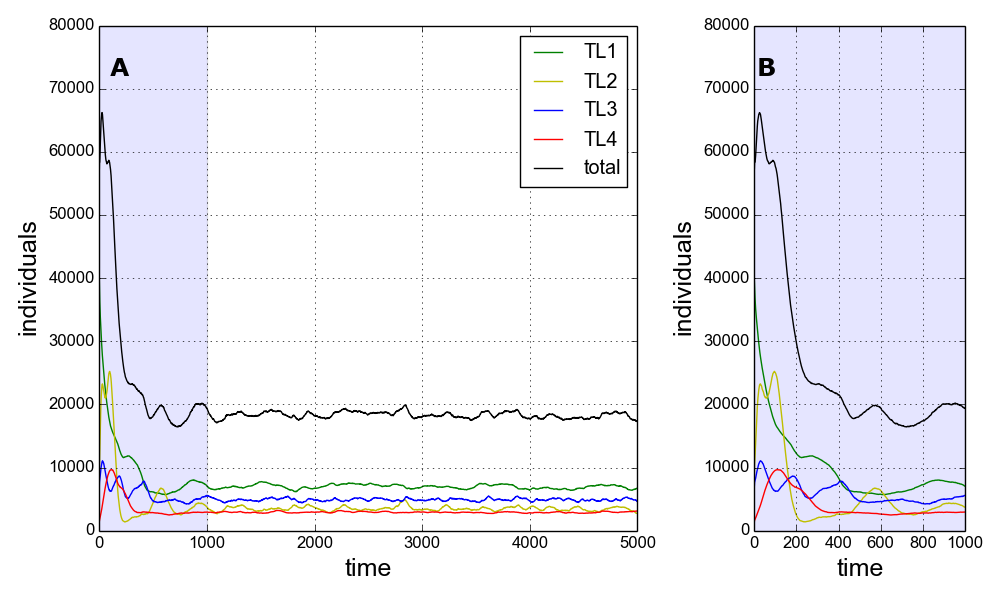
\includegraphics[width=\textwidth]{{{random_plots/example_trophic_dynamics_default}}}
	\caption[Community dynamics by trophic level.]{Example of community dynamics by trophic level, simulated using the IBM with \emph{default parameters}. No habitat loss. Antagonistic community: $MAI=0.0$. (A) The full dynamics for 5000 time steps. (B) Magnification of the first 1000 time steps, containing initial transience.}
	\label{fig:example_model_dynamics}
\end{figure}
%% figures produce by plot_trophic_dynamics.py in random_plots/ (have to copy .csv files locally)
\begin{figure}
	\centering
	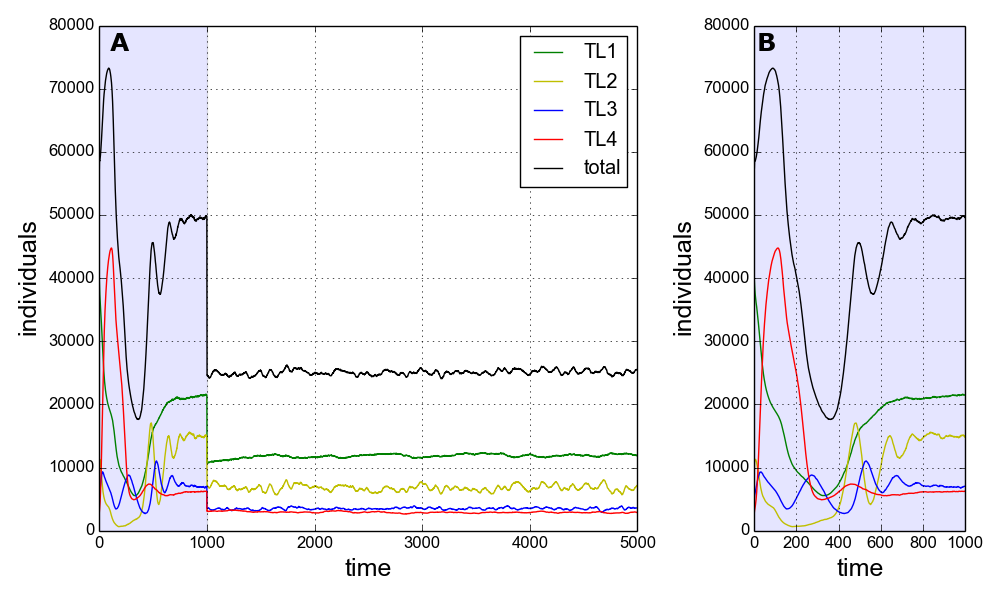
\includegraphics[width=\textwidth]{{{random_plots/example_trophic_dynamics_default_HL40_mai1}}}
	\caption[Community dynamics by trophic level, with mutualism and habitat loss.]{Similar to figure \ref{fig:example_model_dynamics}, but with $MAI=1.0$, and with $40\%$ contiguous habitat loss applied on the 1000th time step.}
	\label{fig:example_model_dynamics_HL40}
\end{figure}

\begin{figure}[p]
	\centering
	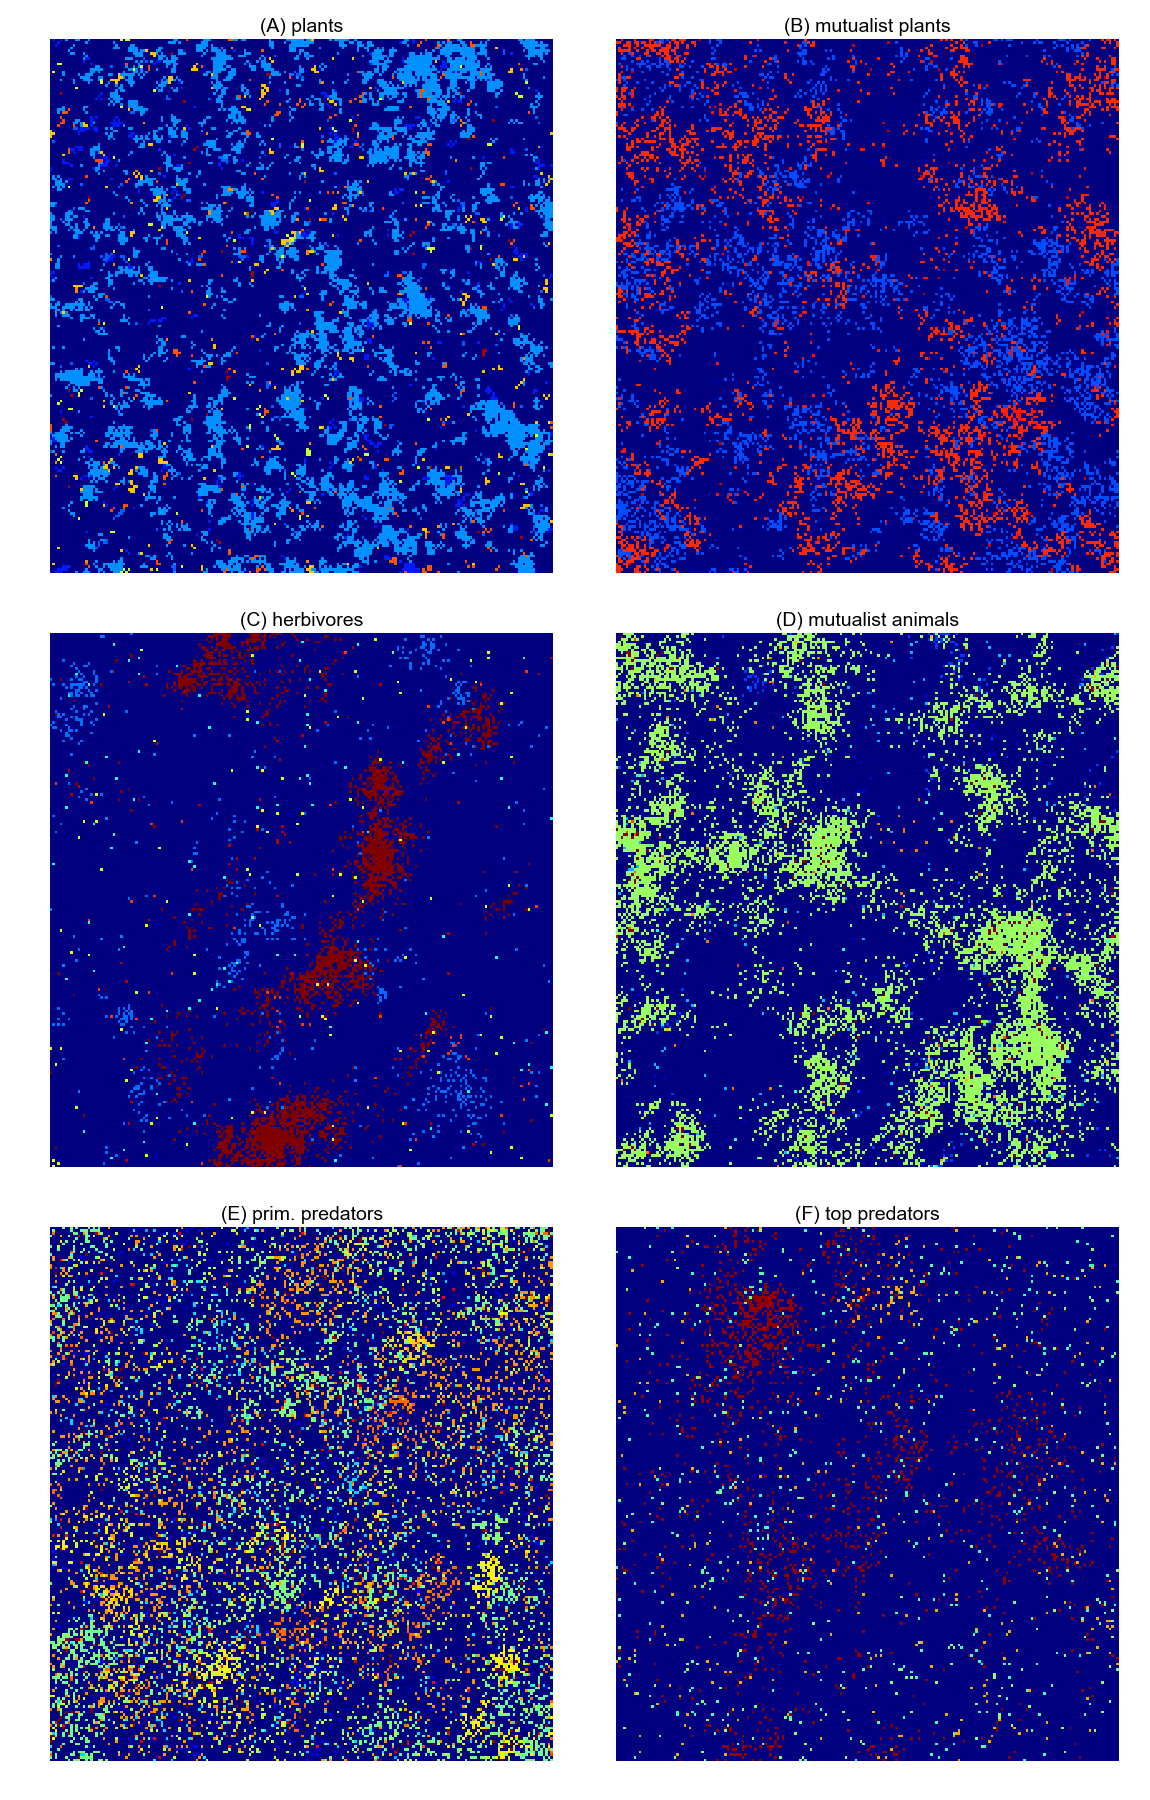
\includegraphics[width=0.8\textwidth]{{{random_plots/space/spatial_state_mai0.5}}}
	\caption[Spatial depiction of IBM community.]{A spatial representation of each functional group. Each panel (A-F) shows the full landscape ($200 \times 200$ cells). Dark blue represents empty cells. Other colours indicate presence of an individual, coloured by species. $MAI=0.5$, $HL=0\%$.}
	\label{fig:spatial_state_mai0.5}
\end{figure}

Figure \ref{fig:spatial_state_mai0.5} shows the spatial state of the system on the 5000$^{th}$ time step, for a community with $MAI=0.5$. There is no HL. Obviously we cannot generalise from a single image. However observing the communities in space does provide intuition about the dynamics and other properties of interest. For example the community shown displays visibly higher aggregations in the lower two trophic levels (panels A-D) than in the top two (panels E-F). It also appears that the more aggregated species are the most abundant. Such insights, gained from \emph{watching} the system, feed into the analysis and discussion (at least implicitly) throughout the thesis. I have also produced \emph{animations} of the spatial dynamics under various conditions which can be viewed at \cite{mcwilliams2015anim}, and are referenced at relevant points in the thesis.

\section{Ecological metrics and analysis methods}
\label{sec:metrics_explained}

In this section we introduce the metrics and methods used to analyse simulation output, which are standard tools of community ecology. These methods fall nicely into four categories. \emph{Biodiversity} metrics (section \ref{sec:define_dviersity}) capture some aspect of the diversity of species. \emph{Stability} metrics (section \ref{sec:def_stability_metrics}) try to quantify stability - a task that is fraught with confusion and therefore given some thought here. \emph{Spatial metrics} characterise the properties of the distribution of species in space. \emph{Network metrics} use properties of the \emph{realised} interaction network to provide insight about community structure. The choice of metrics provides a balance across the aforementioned categories, and largely is determined by the analysis previously conducted by Lurgi et al. \cite{lurgi2015effects}. Additionally we present a way to use rank-abundance distributions to measure \emph{evenness} in species abundances (section \ref{sec:define_rads}), and implement several new stability metrics based on \emph{invariability} (section \ref{sec:def_invariability}). In all that follows we use the number of individuals belonging to a species to measure \emph{abundance}. An alternative would be to use \emph{biomass}, which is potentially more informative due to allometric scaling \cite{west1997general}. However biomass information is not included in the model, and number of individuals is a commonly used alternative.

%% Do mention use of abundance rather than e.g. biomass!
% Mention here sampling and steady-state assumption?

%Stability - Jacobian, dynamic stability, multi-stability, CoV, reproductive stability. 
%Robustness - secondary extinctions, cascading effects \cite{evans2013robustness}. Re-wiring algorithms?

\subsection{Biodiversity metrics}
\label{sec:define_dviersity}

\textbf{Species richness} is very simply defined as the number of different species present (in a sample). As discussed in section \ref{sec:intro_habitat_loss}, many HL studies have focused in species richness. However this metric only changes when species become locally extinct, or sufficiently rare that they are not present in samples. Therefore this metric is insensitive to many ways that a community may respond to perturbation. We define the \textbf{relative abundance} of a species $i$ by:
\begin{equation}
r_i = \frac{N_i}{\Sigma_{j=1}^S N_j},
\label{eq:rel_abun}
\end{equation}
%
where $N_i$ is the number of individuals belonging to species $i$, $S$ is the number of species. Unless otherwise stated the sum in \eqref{eq:rel_abun} is taken over all species, such that the relative abundance is the proportion of individuals in the whole community that belong to species $i$. The relative abundance of species within a subset of the whole community (such as a functional group) may also be calculated. In this case the sum is only over the subset of species, giving the abundance relative to the other species in the group. The relative abundance is used to calculate the \textbf{Shannon diversity index}:
\begin{equation}
D_{Sh} = -\Sigma_{i=1}^S r_i log( r_i),
\label{eq:shan_div}
\end{equation}
%
which is simply the Shannon entropy of species relative abundances. Therefore diversity, by this metric is maximal when all species have the same relative abundance, and approaches zero if one species out competes all others. There is no standard convention for base of the logarithm. Throughout this thesis we use the natural logarithm (base $e$) for all information theoretic measures. Normalising $D_Sh$ by the maximum diversity gives us the \textbf{Shannon equitability index}:
\begin{equation}
E_{Sh} = \frac{D_{Sh}}{log(S)},
\label{eq:shan_eq}
\end{equation}
%
since the maximum diversity is equal to the logarithm of the number of species $S$. The metric is constrained between 0 and 1, and is maximal when all species have the same relative abundance. Both the Shannon metrics can be computed for a subsets of the community (for example a functional group) by using the relative abundance within the subset \eqref{eq:rel_abun}, and reducing $S$ accordingly. Throughout the thesis we use only the Shannon equitability index because it controls for the number of species present, and therefore changes in this metric are not driven by changes in species richness that may be induced by HL. Hereafter \emph{we use the terms equitability and diversity interchangeably} to refer to the normalised metric given in \eqref{eq:shan_eq}.  
%Richness, Simpsons, Shannon Entropy

\subsubsection{Rank abundance distributions}
\label{sec:define_rads}

Rank abundance distributions (RADs) provide another tool to study the patterns in species abundances. They are sometimes referred to as Whittaker plots, after his 1965 paper on species abundances in plant communities \cite{whittaker1965dominance}. To construct the RAD, species are simply ranked from most to least abundant, such that the distribution is monotonically decreasing. It is conventional to use the logarithm of the abundance measure when plotting, because of the wide range of abundances often found in nature. We use RADS to \emph{visually inspect} the distribution of species abundances, and to develop \emph{alternative measures of evenness}. Example RADs for simulated communities can be seen in figure \ref{fig:example_rads_random}.

In natural communities it has been observed that RADs tend to be \emph{long-tailed} - with relatively few species of high abundance, and relatively many species of low abundance. As such RADs have often been found to fit well to a \emph{log-normal} distribution \cite{lurgi2015effects,whittaker1965dominance}, or modifications thereof \cite{mcgill2007species}. However numerous alternative models have been proposed \cite{wilson1991methods}, and are implemented in the \emph{vegan} package \cite{oksanen2007vegan} of the programming language \emph{R}. \textbf{We propose two measures of evenness}, calculated by fitting two alternative models to a RAD. We use two models from those available in \emph{vegan}: the \emph{Zipf} and the \emph{preemption} model, because both have a parameter which is easily interpreted as a measure of the evenness of the distribution. The \textbf{Zipf model} is given by the power law: 
% use this package to fit models to RADs constructed from the simulated communities, with the particular goal of determining how the \emph{evenness} of species abundances changes under HL (see predictions in section \ref{sec:intro}). 
\begin{equation}
\hat{a}_r = N\hat{p}_1r^{\gamma}
\label{eq:zipf}
\end{equation}
%
where $\hat{a}_r$ is the predicted abundance of the species rank $r$; $N$ is the total number of individuals; $\hat{p}_1$ is the estimated proportion of the most abundant species (rank 1); and $\gamma \in \mathbf{R}^-$ is the estimated exponent of the power law. So $\gamma$ gives the gradient of the line defined by \eqref{eq:zipf} in log-log space. Therefore a smaller value of $\left| \gamma \right|$ indicates a shallower line and more even distribution of abundances (see for example figure \ref{fig:example_rads_random}). The \textbf{preemption model} is given by a geometric sequence:

\begin{equation}
\hat{a}_r = N\alpha(1-\alpha)^{r-1}
\label{eq:preemption}
\end{equation}
%  
where $\alpha \in [0,1]$ is the single model parameter, and other symbols have the same meaning as in \eqref{eq:zipf}. Therefore the estimated abundance decreases by a fraction $(1-\alpha)$ for each rank, and the choice of $\alpha$ is constrained such that the estimated abundances sum to $N$. In semi-log space, as is used to plot the RADs, the preemption model gives a straight line, since \eqref{eq:preemption} implies:
\begin{equation}
log\left(\hat{a}_r\right) = log\left(1-\alpha\right)r + C,
\label{eq:preemption_line}
\end{equation}
%  
where $C$ is constant. Therefore the smaller the value of $\alpha$, the closer the gradient of the line is to zero, and the more even the distribution of abundances. In our case, as is common \cite{oksanen2007vegan}, we use relative abundances to allow comparison of the RADs between communities with a different total number of individuals. Therefore $N=1$, and $\hat{a}_r$ are fractions, in \eqref{eq:zipf} and \eqref{eq:preemption}. The models are fitted using \emph{R}, and the parameters $\gamma$ and $\alpha$ used as complementary metrics for evenness - in both cases \emph{the smaller the absolute value of the parameter, the more even the distribution of abundances in the community}. As with the Shannon metrics, RADs may be produced for subsets of the community.   


\subsection{Stability metrics}
\label{sec:def_stability_metrics}

There are various different theoretical concepts relating to stability in ecosystems, which can lead to confusion \cite{arnoldi2015,mumby2014ecological}. It is remarkable that complex ecosystems are able to function with relative consistency in the face of extrinsic variability and perturbations (e.g. due to environmental factors and human activity). Ecological theory does not yet fully explain this phenomenon. Donohue et al. \cite{donohue2013dimensionality} explain that stability is a multi-dimensional concept involving related but distinct components such as variability, resilience, robustness and persistence. Communities may appear stable in some respects, but unstable in others, especially under perturbations such as habitat loss. Our main approach to stability focuses on features of temporal population dynamics and is outlined below. However we first introduce two key stability concepts for clarification. \textbf{Persistence} simply means lack of extinction i.e. a population of the species continues to exist through time \cite{dytham1995effect}. In the current context persistence of a species is defined by the presence of individuals belonging to that species in the artificial landscape. This concept plays a key role in chapter \ref{chap:stress_testing}. \textbf{Robustness} is a measure of how resistant a community is to perturbation. It is often used in the context of species extinctions, with robustness metrics measuring the expected extent of cascading extinctions after removal of some species \cite{evans2013robustness}. \textbf{Dynamic stability}, in the current context, refers to properties of the dynamics of the system. Its definition requires further clarification.    

As we saw in section \ref{sec:intro_interactions}, May demonstrated \cite{may1972will} that high connectance and strong interactions in random communities leads to instability. This lead to the conclusion that ecosystem \emph{complexity} reduces stability, which contradicts observations of nature and has been the subject of ongoing debate ever since (see discussion in section \ref{sec:intro_role_of_sturcture}). The measure of stability used in this body of literature is derived from the mathematics of dynamical systems. The assumption is that the dynamics of an ecosystem can be modelled as a system of non-linear ordinary differential equations (ODEs). It is possible to calculate the local stability of the equilibrium state of this system - it is stable if all eigenvalues of the Jacobian have negative real parts. Therefore this commonly used theoretical concept of stability relates to the stability of ecosystem models. It is often referred to as \emph{asymptotic resilience} \cite{arnoldi2015} because the magnitude of the real parts of the eigenvalues determine the rate of return to equilibrium after perturbation. 

Asymptotic resilience is used to measure stability in chapter \ref{chap:interactions}. However, in practical applications, this measure cannot be used because of the difficulty in estimating the elements of the Jacobian from empirical data (see the aforementioned chapter). Therefore empiricists use an alternative measure that can be computed directly from population dynamic time-series \cite{campbell2011experimental, donohue2013dimensionality}. \textbf{Temporal variability} is measured as the coefficient of variation in the abundance time-series of a species. So for species $i$: 
\begin{equation}
CV_i = \frac{\sigma_i}{\mu_i},
\label{eq:cov}
\end{equation}
%
where $\sigma_i$ and $\mu_i$ are the standard deviation and mean of the species abundance respectively, over the time period in question. To derive a community level measure we average $CV_i$ over all species, and in all subsequent analysis refer to the resulting metric as \textbf{mean\_CV}. The metric captures the variability of population dynamics, with the assumption that \emph{higher variability implies lower stability}. However the relationship to asymptotic resilience (AR) is not clear. For example a system may exhibit a limit-cycle which is globally stable such that all trajectories approach it asymptotically (an attractor). Therefore AR classifies the system as stable. However the \emph{mean\_CV} may be high, depending on the amplitude of the limit cycle, suggesting instability. It appears that the two stability concepts are incompatible.


\subsubsection{Invariability}
\label{sec:def_invariability}

%% regarding sync mechanisms: loreau2008species

A group of theoreticians at the \emph{Station d'Ecologie Th\'eorique et Exp\'erimentale} in Moulis are currently attempting the clarify the issues surrounding stability, and characterise the relationship between AR and stability metrics based on variability \cite{arnoldi2015,montoya2016invariability}. Their work is currently restricted to the case of systems with a stable equilibrium point, rather than an attractor. They introduce four new stability metrics based on \emph{invariability}, which are named: ecosystem ($I_{eco}$), population ($I_{pop}$) and minimum invariability ($I_{min}$), and ecosystem synchrony ($Sync$). These are defined, respectively, as follows:
\begin{eqnarray}
I_{eco} &=& \frac{1}{CV(X_{tot})^2}, \\[5pt] 
I_{pop} &=& \frac{(X_{tot}^*)^2}{(\Sigma_i \sqrt{Var(X_i)})^2}, \\[5pt]
I_{min} &=& \underaccent{i}{min} \frac{(X_i^*)^2}{Var(X_i)}, \\[5pt]
Sync    &=& \frac{Var(X_{tot})}{(\Sigma_i \sqrt{Var(X_i)})^2},\label{eq:def_eco_sync}
\end{eqnarray}
where $X_i$ is the abundance time-series vector of species $i$; $X_{tot}$ is the total abundance time-series (i.e.  $\Sigma_i X_i$);  $CV$ is the coefficient of variation (as defined in \eqref{eq:cov}); and $X_i^*$, $X_{tot}^*$ are the species level and total abundance values of the stable equilibrium point respectively. Therefore $I_{eco}$ is the squared inverse of the metric $mean\_CV$, whilst $I_{min}$ is the squared inverse of the coefficient of variation of the \emph{most variable species}. $I_{pop}$ is a weighted sum of the species level invariabilities, and $Sync$ is given by the ratio $I_{pop} / I_{eco}$. In \cite{montoya2016invariability} it is shown that AR is strongly dependent on species composition, and is closely related to $I_{min}$ - it is often dominated by the least abundant and most variable species. Therefore they conclude that AR is not a reliable metric, and advocate some combination of invariability metrics to characterise stability. We implement and test these metrics in our analysis (chapter \ref{chap:habitat_loss_high_immigration}), and note here the following relevant properties:

\begin{itemize}
	\item $I_{eco}$ is a measure of system level stability, and should behave similarly to $mean\_CV$.
	\item $I_{min}$ is the stability of the most variable species, which is often the least abundant \cite{montoya2016invariability}
	\item $I_{pop}$ is weighted in favour of the more abundant species, to reduce sensitivity to very rare species.
	\item $Sync$ is always less than or equal to one. If all species abundances vary in perfect synchrony $Sync=1$. However any deviation from synchrony results in some cancellation in variability when abundance is aggregated over species, meaning that invariability is greater at the ecosystem level, than when summed over species i.e. $Sync<1$.
\end{itemize}

\subsection{Spatial metrics}
\label{sec:def_spatial_metrics}

The spatially explicit nature of the IBM allows us to study the spatial structure of the communities. We use the spatial-autocorrelation metrics Moran's I and Geary's C to measure aggregation in species spatial distributions \cite{dale2014spatial, lurgi2015effects}. \textbf{Moran's I} is a measure of global correlation, and for a single species $s$ is given by:
\begin{equation}
MI_s = \frac{N}{\Sigma_{i=1}^N \Sigma_{j=1}^N w_{ij}}  \frac{\Sigma_{i=1}^N \Sigma_{j=1}^N w_{ij}(X_i - \bar{X})(X_j - \bar{X})}{\Sigma_{i=1}^N (X_i - \bar{X})^2},
\label{eq:morans}
\end{equation}
%
where $N$ is the total number of cells; $X_i$ is equal to 1 if the species is present in cells $i$ and equal to 0 if not; $\bar{X}$ is the mean of $X_i$ over all cells; and $w_{ij}$ is spatial weight between cells $i$ and $j$. We take $w_{ij}$ equal to 1 if the cells are neighbours (distance-1), and 0 otherwise. In the extreme of total aggregation, when every cell containing the species is surrounded by other cells containing the species, $MI_s=1$. In the opposite extreme, when no cells containing the species are adjacent to each other, $MI_s=-1$. For a random distribution of individuals the expected value $E(MI_s) = -1/(N-1)$, which is close to zero for large $N$. For a single species $s$, \textbf{Geary's C} is given by:
\begin{equation}
GC_s = \frac{(N-1)\Sigma_{i=1}^N \Sigma_{j=1}^N w_{ij}(X_i - X_j)^2}{2W \Sigma_{i=1}^N (X_i - \bar{X})^2},
\label{eq:gearys}
\end{equation}
%
where $W$ is the sum over all $w_{ij}$, and all other symbols have the same meaning as in \eqref{eq:morans}. GC is a measure of local aggregation and is constrained between maximum aggregation at $GC_s=0$, and minimum aggregation at $GC_s=2$. The expected value for a random distribution is $E(GC_s)=1$, indicating no local correlation structure. To obtain community level metrics, the species level aggregation values are averaged over all species. In \cite{lurgi2015effects} the aggregation metrics were associated with stability, since higher aggregation may confer species with greater reproductive stability and reduced vulnerability to predation. However this relationship is not concrete.

Three further spatial metrics are used to characterise species \emph{spatial ranges}. The \textbf{species range centroid} is calculated as the two-dimensional centre of mass of all individuals on the lattice. The \textbf{species range area} is calculated as the area of the circle, centred on the centroid, that contains $97\%$ of the individuals of that species. \textbf{Species density} is then defined as the number of individuals divided by the area of the range. These three metrics are used to calculate the temporal variability of species spatial ranges, by taking the coefficient of variation in each metric (as defined in \eqref{eq:cov}) over the time period of interest. The coefficients of variation are averaged over all species to obtain \textbf{community level metrics for spatial variability}: $mean\_CV\_centroid$, $mean\_CV\_area$, and $mean\_CV\_density$. These metrics provide an interesting comparison with variability in species abundance, and represent another alternative component of system stability.


\subsection{Network metrics}
\label{sec:define_network_metrics}

The importance of the structure of the interaction network in determining the high level patterns and functions of an ecological community was discussed in section \ref{sec:intro_role_of_sturcture}. A wide range of \emph{qualitative} and \emph{quantitative} descriptors are available to characterise the structure of the interaction network \cite{bluthgen2008interaction, lurgi2015effects, tylianakis2007habitat,bersier2002quantitative}. Qualitative metrics refer to those that depend only on the presence/absence of links i.e they are used on unweigthed networks. Quantitative metrics refer to those that use some measure of interaction strength i.e. a weighted network. It has been shown that the quantitative metrics are less sensitive to sampling intensity and generally more reliable than their qualitative counterparts \cite{banavsek2004sampling, bluthgen2006measuring}. Also Tylianakis and collaborators have shown \cite{tylianakis2007habitat} that quantitative metrics may be required in order to detect the effects of habitat degradation on ecological communities (host-parasitoid networks in their study). In our analysis we use the same metrics as in \cite{lurgi2015effects}, which are defined below.


\subsubsection{Qualitative network descriptors}
\label{sec:def_qual_metrics}

The unweighted interaction network is defined by the asymmetric adjacency matrix $\mathbf{a}$, where element $a_{ij}$ is 1 if there exists a trophic link from prey $i$ to predator $j$, and 0 otherwise. The \textbf{connectance} is defined as:
\begin{equation}
C = L/S^2,
\label{eq:connectance}
\end{equation}
%
where $L$ is the number of links (non-zero elements in $\mathbf{a}$), and $S$ is the number of species. Qualitative \textbf{generality} (G) and \textbf{vulnerability} (V) are defined as the mean number of prey per predator, and the mean number of predator per prey respectively. These are given by
\begin{eqnarray}
G &=& \frac{L}{N_B + N_I}, \\[5pt]
V &=& \frac{L}{N_I + N_T}, 
\end{eqnarray}
%
where $N_B$, $N_I$ and $N_T$ are the number of species belonging to basal, intermediate and top trophic levels respectively. \textbf{Compartmentalisation} is a measure of how frequently species share common neighbours, and is given by:
\begin{equation}
P = \frac{1}{S(S-1)} \Sigma_{i=1}^S \Sigma_{j \neq i} c_{ij},
\label{eq:copart}
\end{equation}
%
where $c_{ij}$ is the number of species with which both $i$ and $j$ interact divided by the number of species with which either $i$ or $j$ interact \cite{lurgi2015effects}. Finally \textbf{nestedness} is a measure of the extent to which the diets of specialist species are subsets of the diets of more generalist species \cite{lurgi2015effects} (see figure \ref{fig:nested}). As discussed in section \ref{sec:intro_role_of_sturcture} this is may be an important feature of mutualistic networks. Therefore nestedness is calculated for the mutualistic sub-network only, using the \emph{NODF} algorithm of Almeida-Neto et al. \cite{almeida2008consistent}.

\subsubsection{Quantitative network descriptors}
\label{sec:def_quant_metrics}

The quantitative network metrics used are based on the \emph{Shannon entropy} of link weights - analogous to the way it is used to measure diversity of species abundances. It is common practice to use interaction frequency to define link weights \cite{lurgi2015effects,tylianakis2007habitat,bluthgen2006measuring}, in part because this is easier to measure empirically than, for example, biomass flow. We present here the standard definitions of the Shannon network metrics using the notation of Bersier et al. \cite{bersier2002quantitative}. As previously, the natural logarithm is used for all metrics. It is necessary in what follows to define $0log(0)=0$, which is equivalent to excluding zero elements in the interaction matrix from the calculations. Also rows or columns with sum equal to zero are removed, to avoid division by zero.    
 
The asymmetric weighted matrix of interaction frequencies is denoted by $\mathbf{b}$, where element $b_{ij}$ is the number of individuals of species $i$ consumed by species $j$ during the sampling period. Therefore we can define interaction diversities for the links coming into a species $k$ from its prey, and the links going from $k$ to its predators:  

\begin{eqnarray}
H_{N,k} &=& -\Sigma_{i=1}^{s} \left( \frac{b_{ik}}{b_{\bullet k}} log \left( \frac{b_{ik}}{b_{\bullet k}} \right) \right) \label{eq:prey_div} \\
H_{P,k} &=& -\Sigma_{j=1}^{s} \left( \frac{b_{kj}}{b_{k\bullet}} log \left( \frac{b_{kj}}{b_{k\bullet}} \right) \right) \label{eq:pred_div}
\end{eqnarray}
%
where $H_{N,k}$ is the diversity of inflows from prey; $H_{P,k}$ is the diversity of outflows to predators; $s$ is the total number of species; and $b_{\bullet k}$, $b_{k\bullet}$ are column and row sums giving the total number of interactions that species $k$ has with its prey and predators respectively. The interaction diversity metrics behave just as the Shannon entropy - the higher the number of interaction partners and the more even the interaction frequencies across these partners, the higher the interaction diversities. The exponents of \eqref{eq:prey_div} and \eqref{eq:pred_div} are used to calculate the \emph{effective number} of prey and predators respectively:

\begin{eqnarray}
n_{N,k} &=& \begin{cases} e^{H_{N,k}}  \\ 0 \mbox{     if } b_{\bullet k}=0 \end{cases} \label{eq:effective_prey} \\
n_{P,k} &=& \begin{cases} e^{H_{P,k}}  \\ 0 \mbox{     if } b_{k\bullet}=0 \end{cases} \label{eq:effective_pred}
\end{eqnarray}
%
where the symbols have the same meaning previously. These metrics have the property that if the interaction frequencies of species $k$ are distributed equally amongst its interaction partners, then the effective number of prey/predators is equal to the actual number. However, if the interaction frequencies are not equal between partners, the effective number of prey/predators is reduced, since there is some preferential interaction. These effective number of species are used to calculate \textbf{weighted quantitative generality and vulnerability}, which are defined as:  
\begin{eqnarray}
G_q &=& \Sigma_{k=1}^{s} \left( \frac{b_{\bullet k}}{b_{\bullet \bullet }} n_{N,k} \right) \label{eq:G_q} \\
V_q &=& \Sigma_{k=1}^{s} \left( \frac{b_{k\bullet }}{b_{\bullet \bullet }} n_{P,k} \right) \label{eq:V_q}
\end{eqnarray}
%
where $b_{\bullet \bullet }$ is the total number of interactions. So the metrics in \eqref{eq:G_q} and \eqref{eq:V_q} give a weighted average of the effective numbers of prey and predators respectively. They are weighted by the fraction of the total interactions the species $k$ is involved, such that species with more interactions contribute most to the average.

We also calculate metrics for \textbf{interaction diversity} ($H2$) and \textbf{specialisation} ($H2'$). These are applied to the mutualistic sub-network only because the specialisation metric $H2'$ is implemented in \emph{R} in the \emph{bipartite} package \cite{dormann2008introducing}. (It may be possible that a multi-trophic version of the specialisation metric can be derived.) We define:
\begin{equation}
p_{ij} = \frac{\Sigma_{j=1}^S b_{ij}}{ \Sigma_{i=1}^S \Sigma_{j=1}^S b_{ij}},
\end{equation} 
%
as the proportion of the total number of interactions which occur between prey $i$ and predator $j$. Then the interaction diversity is given by:
\begin{equation}
H2 = - \Sigma_{i=1}^S \Sigma_{j=1}^S p_{ij} log(p_{ij}),
\label{eq:h2}
\end{equation}
%
which is maximal when all interactions between prey and predator have the same frequency i.e. the distribution of interaction frequencies is most even. The specialisation metric ($H2'$) is obtained by standardising $H2$ with respect to the theoretical maximum and minimum diversity:
\begin{equation}
H2' = \frac{H2_{max} - H2}{H2_{max} - H2_{min}},
\label{eq:h2_prime}
\end{equation}
% 
where $H2_{max}$ and $H2_{min}$ are the extremes of the diversity values that can be achieved if the total number of interactions of each species is held constant. As such $H2'$ is equal to 0 and 1 for maximum generalisation and specialisation respectively. We calculate $H2'$ using the \emph{bipartite} package in \emph{R}.


\subsubsection{Interaction strength metrics}
\label{sec:def_iss}
A key feature of ecological communities, and a central theme of this thesis, is the strength of interactions between species. As with stability (section \ref{sec:def_stability_metrics}), there are numerous ways to define the strength on an interaction \cite{berlow2004interaction}. We have already seen that interaction frequency ($b_{ij}$) serves as one proxy for interaction strength. In the IBM we may expect that the frequency of an interaction will be largely determined by the abundances of the interacting species. If two species are very abundant then the individuals of these two species are more likely to encounter each other in space. However other factors may contribute. The distribution of species in space may affect how often they interact. For example two species may be abundant but highly aggregated in different regions of the landscape, and so are unable to interact. Factors such as competition and stochasticity may also influence interaction frequencies.   

In addition to frequency we define an interaction strength metric $IS$, which for the interaction between species $i$ and $j$ takes the value:
\begin{equation}
IS_{ij} = \frac{b_{ij}}{N_iN_j},
\label{eq:is3}
\end{equation}
%
and as such represents the per-capita effect of a predator, per-capita of prey. In subsequent analysis $IS$ refers to the mean value of \eqref{eq:is3} over all interactions in the network. This metric is useful because it is analogous to the Lotka-Volterra interaction coefficients and their generalisation to other ODE population dynamic models \cite{berlow2004interaction}. We return to look in more detail at this metric and its interpretation in chapter \ref{chap:interactions}.
